\documentclass[../main.tex]{subfiles}
\begin{document}
\chapter{More CLIPT Sanity Checks}\label{app:clipt-sanity}

We performed a number of additional  sanity checks to guide our choices around the design of CLIPT.

\section{Why not just CLIP?}

\begin{figure}[t]
	\centering
	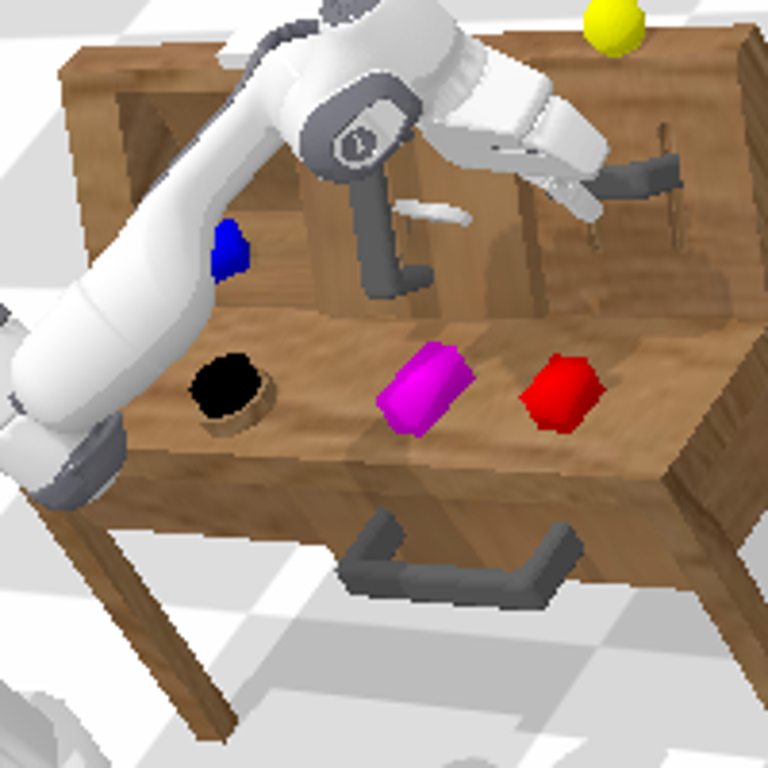
\includegraphics[width=0.49\textwidth]{figures/clip_ood/calvin_env_original}
	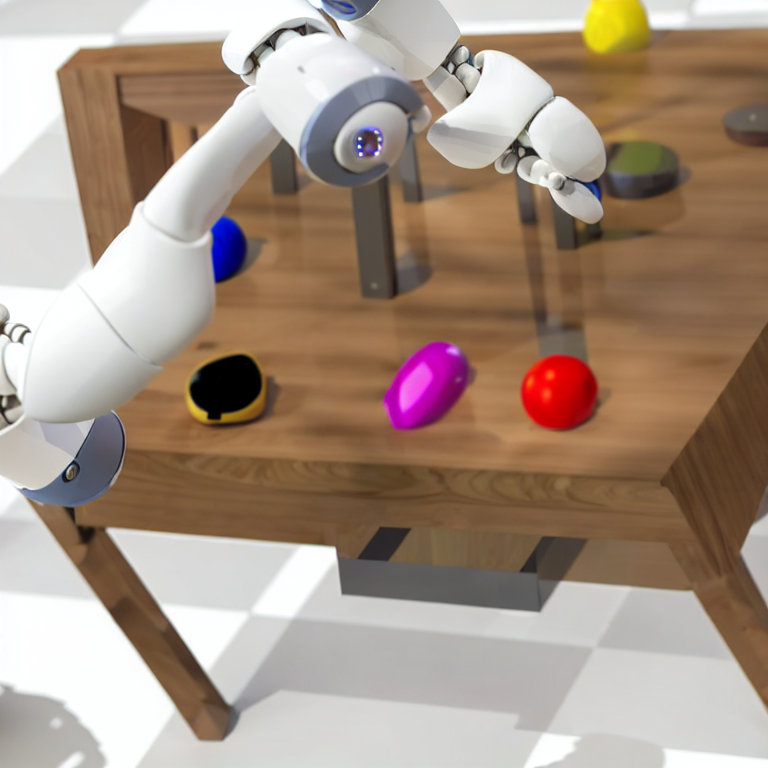
\includegraphics[width=0.49\textwidth]{figures/clip_ood/calvin_env_realistic}
	\caption[Original and "Realistic" CALVIN state]{Comparison of an image from the CALVIN environment and the corresponding ``realistic''
		version obtained via latent diffusion}
	\label{fig:sd-realistic}
\end{figure}

CLIPT modifies CLIP such that there are two separate MLPs projecting concatenated representations
back into the original dimension. This choice is not arbitrary. Indeed, a more comfortable choice
would have been to use the representations from CLIP's vision and text encoders directly. As
outlined in the previous chapter, we are motivated to make this design decision for two reasons:

\begin{enumerate}
	\item We define a trajectory to be composed of \emph{at least} start and end state, necessitating
	      the need for two-image representations.
	\item We believe images of our state will be slightly out of domain compared to CLIP's training
	      mixture.
\end{enumerate}

We take the first as a definitional aspect, a basic premise, for which we therefore do not envision
verification as being necessary. We however do perform a quick experiment to check the validity of
our second motivation. We expect the similarity between textual annotations and images of our state
to be lower than the similarity between textual annotations and more "realistic" images, which are
closer to the distribution of data CLIP was trained on. To test this hypothesis, we collect
8 textual annotations and 8 images of final states of the corresponding trajectories. We compute the
cosine similarity between the CLIP representations of all possible pairings, for a total of 64
similarity values. We then repeat this computation, replacing the images with "realistic" versions
obtained via an off-the-shelf text-conditioned image-to-image model. In particular, we use
RunwayML's "Stable Diffusion 1.5" checkpoint of \citet{rombach_high-resolution_2022}'s latent
diffusion model\footnote{Courtesy of RunwayML: \href{https://runwayml.com/}{runwayml.com}}. Using
the HuggingFace diffusers library \citep{von_platen_diffusers_2023}, we set strength to
0.35, guidance scale to 50 and employ the following prompt: ``\textit{Photograph of robotic arm
	interacting with wooden table top. Canon 60D. Realistic, HD, 8k, ultra detailed.}'' Figure
\ref{fig:sd-realistic} presents a sample comparison between an original state image and its
``realistic'' version. Table \ref{tab:clip-ood-check} instead summarizes the results of the
experiment.

\begin{table}[tb]
	\centering
	\caption[Original and ``Realistic'' CALVIN Similarity]{Similarity statistics between textual
		annotations and original vs ``realistic'' state images.}
	\label{tab:clip-ood-check}
	\begin{tabular}{@{}rcc@{}}
		\toprule
		Cosine Similarity & Original state image & ``Realistic'' state image \\ \midrule
		mean              & 0.308                & 0.350                     \\
		median            & 0.311                & 0.353                     \\
		maximum           & 0.384                & 0.408                     \\
		minimum           & 0.234                & 0.289                     \\
		std. err.         & 0.004                & 0.003                     \\ \bottomrule
	\end{tabular}
\end{table}

We find that there is a clear difference in the similarity of textual annotations and the original
state images and the similarity of textual annotations and the transformed ``realistic'' state
images. In particular, we find the latter case to result in clearly higher similarity. While far
from a perfect evaluation, we take this as sufficient evidence that some fine-tuning is necessary to
adjust the domain-gap between the CLIP pre-training mixture and our environment state. An
alternative solution may have been to simply apply the ``realism'' transform to our environment
state. This is however infeasible for three reasons. Firstly, latent diffusion inference is
computationally expensive. Secondly, there is a very high variance in the results obtained due to
the nature of prompting, resulting in images that rarely preserve the details necessary for the
task. See for instance Figure \ref{fig:sd-realistic}, where the ``realistic'' version loses the any
notion of the sliding door or switch. Lastly, we are still motivated by our first reason above, i.e.
the need for two-image representations, so we will need to train a head on top of CLIP regardless.


\section{Alternatives to CLIPT}

We performed a number of experiments similar to the previous section before choosing to embark on
our modification of CLIP into CLIPT. Our experiments generally consisted in collecting language
annotations and trajectory end states and visualizing similarity matrices in search of well-defined
diagonals. The lack of a diagonal would indicate that whatever modification we were testing in that
experiment was insufficient to guarantee that we could perform our desired swapping of visual goals
language goals. We first tried two alternatives to CLIP, namely FLAVA~\citep{singh_flava_2022} and
ALIGN~\citep{jia_scaling_2021}, however these did not return promising results. We therefore
returned to CLIP and attempted some prompt engineering~\citep{liu_pre-train_2023,
	gu_systematic_2023} of the natural language instructions. Specifically we tried converting the
instructions to the past tense, paraphrasing them to be more similar in style to image captions, and
finally even some BLIP2-based~\citep{li_blip-2_2023} reformulations. Ultimately however, none of
these experiments provided satisfactory results, so we proceeded with our CLIPT modifications.

\section{Task Classifier}

Before proceeding to our GCBC implementation, we wanted to check whether our idea of training on
visual representations and evaluation on textual representations from CLIPT was sound on an easier
task. Leveraging the fact that CALVIN trajectories annotated with language are additionally also
annotated with the task that is being completed, we implemented a simple task classifier network.
This consisted in a simple three-linear-layer MLP, trained to classify visual representations of
CLIPT across the 34 possible tasks. We used CLIPT-1P, the checkpoint of CLIPT from the first phase
of training where the language encoder is simply the CLIP language encoder. At test time, we then
evaluated with both visual and textual trajectories and compared the performance across modalities.
We report the results in Table~\ref{tab:task-classifier}.

\begin{table}[tb]
	\centering
	\caption[The test accuracy of our task classifier.]{The test accuracy of our task classifier on
		visual trajectory representations and textual trajectory representations from CLIPT-1P.}
	\label{tab:task-classifier}
	\begin{tabular}{@{}rcc@{}}
		\toprule
		                                            & \textbf{Accuracy} & \textbf{Std. Err.} \\ \midrule
		\textbf{Visual Trajectory Representations}  & 0.703             & 0.003              \\
		\textbf{Textual Trajectory Representations} & 0.857             & 0.009              \\ \bottomrule
	\end{tabular}
\end{table}

To our great surprise, the classifier performed better when classifying textual trajectory
representations than when classifying visual trajectory representations, despite being trained on
the latter. One possible explanation is that the frames and/or trajectories in the test set are
somewhat out of distribution compared to those in the train split, while the textual descriptions do
not really change too much between splits. You explanation was somewhat reinforced when noticing
that textual accuracy remained almost unchanged between validation and test ($\sim 0.85$) while
visual accuracy dropped from 0.89 in validation to 0.70 in test. Given the promising results with
our task classifier, we proceeded with our GCBC implementation.

\chapter{More GCBC experiments}
\section{Performance over training}

In an attempt to diagnose the relatively underwhelming performance of our policy, we perform our
evaluation on the test set at various checkpoints throughout training on the CALVIN dataset. Figure
\ref{fig:gcbc-sr-curve} presents the mean SR over training when conditioning on textual trajectory
representations\footnote{We mistakenly performed these evaluations without context resets. However,
	since we are mainly interested in the trend rather than actual values with this experiment, we
	deemed this oversight as negligible.}. From the few data-points that we have, we see a very slow
increase in performance over training, indicating that perhaps our model is not sufficiently
expressive. A more complete analysis is however necessary to make conclusions.

\begin{figure}[htb]
	\centering
	\includegraphics[width=\textwidth]{figures/sr_train_curve}
	\caption{GCBC success rate over training}
	\label{fig:gcbc-sr-curve}
\end{figure}

\ifSubfilesClassLoaded{%
	\bibliographystyle{\subfix{bibstyle}}
	\bibliography{\subfix{references-bibtex}}%
}{}

\end{document}
